% Fig. 1 -- Composition of the OLED user interface: two cascaded state machines.
% Source: firmware/esp32c3_oled_mqtt/esp32c3_oled_mqtt.ino (loop() -> loopOled() -> handleButton()).
\documentclass[border=4pt]{standalone}
\usepackage{mathptmx}
\usepackage{amsmath}
\usepackage{tikz}
\usetikzlibrary{positioning,arrows.meta,calc,fit,backgrounds}
\begin{document}
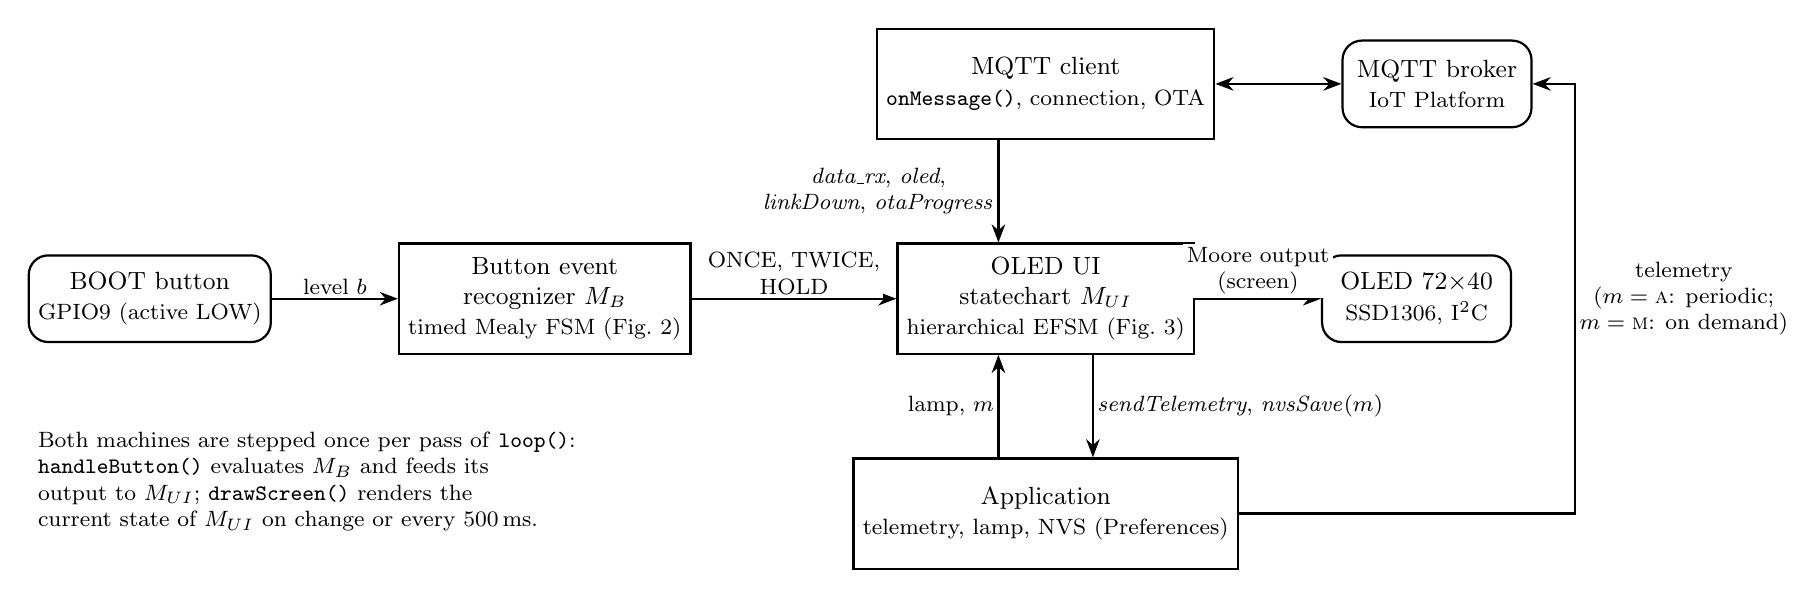
\begin{tikzpicture}[
    >={Stealth[length=2.3mm]}, thick, node distance=1.2cm and 1.6cm,
    blk/.style={draw, minimum height=14mm, minimum width=27mm, align=center, font=\small, fill=white},
    io/.style={draw, rounded corners=7pt, minimum height=11mm, minimum width=24mm, align=center, font=\small},
    lab/.style={font=\footnotesize, align=center, fill=white, inner sep=1.2pt}]
  \node[io]  (btn) {BOOT button\\ \footnotesize GPIO9 (active LOW)};
  \node[blk, right=of btn] (mb)  {Button event\\ recognizer $M_B$\\ \footnotesize timed Mealy FSM (Fig.~2)};
  \node[blk, right=2.6cm of mb] (mui) {OLED UI\\ statechart $M_{UI}$\\ \footnotesize hierarchical EFSM (Fig.~3)};
  \node[io, right=of mui] (oled) {OLED 72$\times$40\\ \footnotesize SSD1306, I$^2$C};
  \node[blk, above=1.3cm of mui, minimum width=40mm] (mqtt) {MQTT client\\ \footnotesize \texttt{onMessage()}, connection, OTA};
  \node[blk, below=1.3cm of mui, minimum width=40mm] (app) {Application\\ \footnotesize telemetry, lamp, NVS (Preferences)};
  \node[io, right=1.6cm of mqtt] (broker) {MQTT broker\\ \footnotesize IoT Platform};

  \draw[->] (btn) -- node[lab, above] {level $b$} (mb);
  \draw[->] (mb) -- node[lab, above] {ONCE, TWICE,\\ HOLD} (mui);
  \draw[->] (mui) -- node[lab, above] {Moore output\\ (screen)} (oled);
  \draw[->] ([xshift=-6mm]mqtt.south) -- node[lab, left] {\textit{data\_rx}, \textit{oled},\\ \textit{linkDown}, \textit{otaProgress}} ([xshift=-6mm]mui.north);
  \draw[->] ([xshift=6mm]mui.south) -- node[lab, right] {\textit{sendTelemetry}, \textit{nvsSave}($m$)} ([xshift=6mm]app.north);
  \draw[->] ([xshift=-6mm]app.north) -- node[lab, left] {lamp, $m$} ([xshift=-6mm]mui.south);
  \draw[<->] (mqtt) -- (broker);
  \coordinate (rr) at ($(oled.east)+(0.8,0)$);
  \draw[->] (app.east) -| (rr |- oled) node[lab, right, pos=1] {telemetry\\ ($m=\textsc{a}$: periodic;\\ $m=\textsc{m}$: on demand)} |- (broker.east);
  \node[font=\footnotesize, align=left, anchor=north west] at ($(btn.south west)+(0,-1.0)$)
    {Both machines are stepped once per pass of \texttt{loop()}:\\
     \texttt{handleButton()} evaluates $M_B$ and feeds its\\ output to $M_{UI}$;
     \texttt{drawScreen()} renders the\\ current state of $M_{UI}$ on change or every 500\,ms.};
\end{tikzpicture}
\end{document}
